\documentclass[12pt,a4paper]{article}
\usepackage[utf8]{inputenc}
\usepackage[german]{babel}
\usepackage[T1]{fontenc}
\usepackage{amsmath}
\usepackage{amsfonts}
\usepackage{amssymb}
\usepackage{graphicx}
\usepackage[left=2.5cm,right=2.5cm,top=2cm,bottom=2cm]{geometry}
\usepackage{float}
\author{Gruppe C14 \\ Julián Häck, Martin Koytek, Lars Wenning, Erik Zimmermann}
\begin{document}
\section{Bestimmung der Schallgeschwindigkeit durch Vermessen einer stehenden Welle}
\subsection{Versuchsbeschreibung}
In diesem Versuch werden wir den Wert der Schallgeschwindigkeit über das Vermessen einer stehenden Welle bestimmen. Der Zusammenhang zwischen der Position der Bäuche der stehenden Welle, der angeregten Resonanzfrequenz und der Schallgeschwindigkeit wird durch folgende Formel beschrieben:
\begin{equation}
v_{Schall} = \lambda\cdot f
\end{equation}
Wir werden den Schalldruck an verschiedenen Stellen innerhalb des Rohres bei einer stehenden Welle messen. Danach tragen wie die Amplitude des Schalldrucks gegen die Strecke auf und suchen die Extrema. Diese Punkte werden dann in einer Linearen Regression verwendet. Die Steigung gibt uns $\frac{\lambda}{2}$ zurück, daraus können wir dann zusammen mit der bereits eingestellten Frequenz die Schallgeschwindigkeit berechnen.

\subsection{Versuchsaufbau und Durchführung}
Verwendete Geräte:
\begin{itemize}
\item Frequenzgenerator
\item Sensor-Cassy
\item Richtmikrofon
\item Lautsprecher
\item Rohr ($0.425\, m \pm 0.001\,$m (Messfehler auf Massband))
\item Massband ($\sigma_{Massband} = 0.001\, m$)
\end{itemize}
Wir haben unser Cassy mit folgenden Einstellungen verwendet:
\begin{itemize}
\item Kanal A / Spannung UA1 / $-10..10\, V$ /
\item Kanal B / Timerbox / Frequenz fb1(E) / $5000\, Hz$ / Torzeit: $1\, s$
\item manuelle Messung
\item Darstellung: X-Achse n / Y-Achse Ua1
\end{itemize}
Den Frequenzgenerator haben wir wie folgt eingestellt:
\begin{itemize}
\item Signalform / $\sim$ (Sinusschwingung)
\item Bereich / $x1k (0.2 - 2.4 x 1\, $kHz$)$
\item $\sigma_f = 10\,$Hz (Abschätzung durch ungenaue Feinabstimmung, gerätbedingt)
\item Offset / 0
\item Amplitude / mittig
\end{itemize}
Die Raumtemperatur betrug $23^{\circ}\, C$.
\begin{figure}[H]
\centering
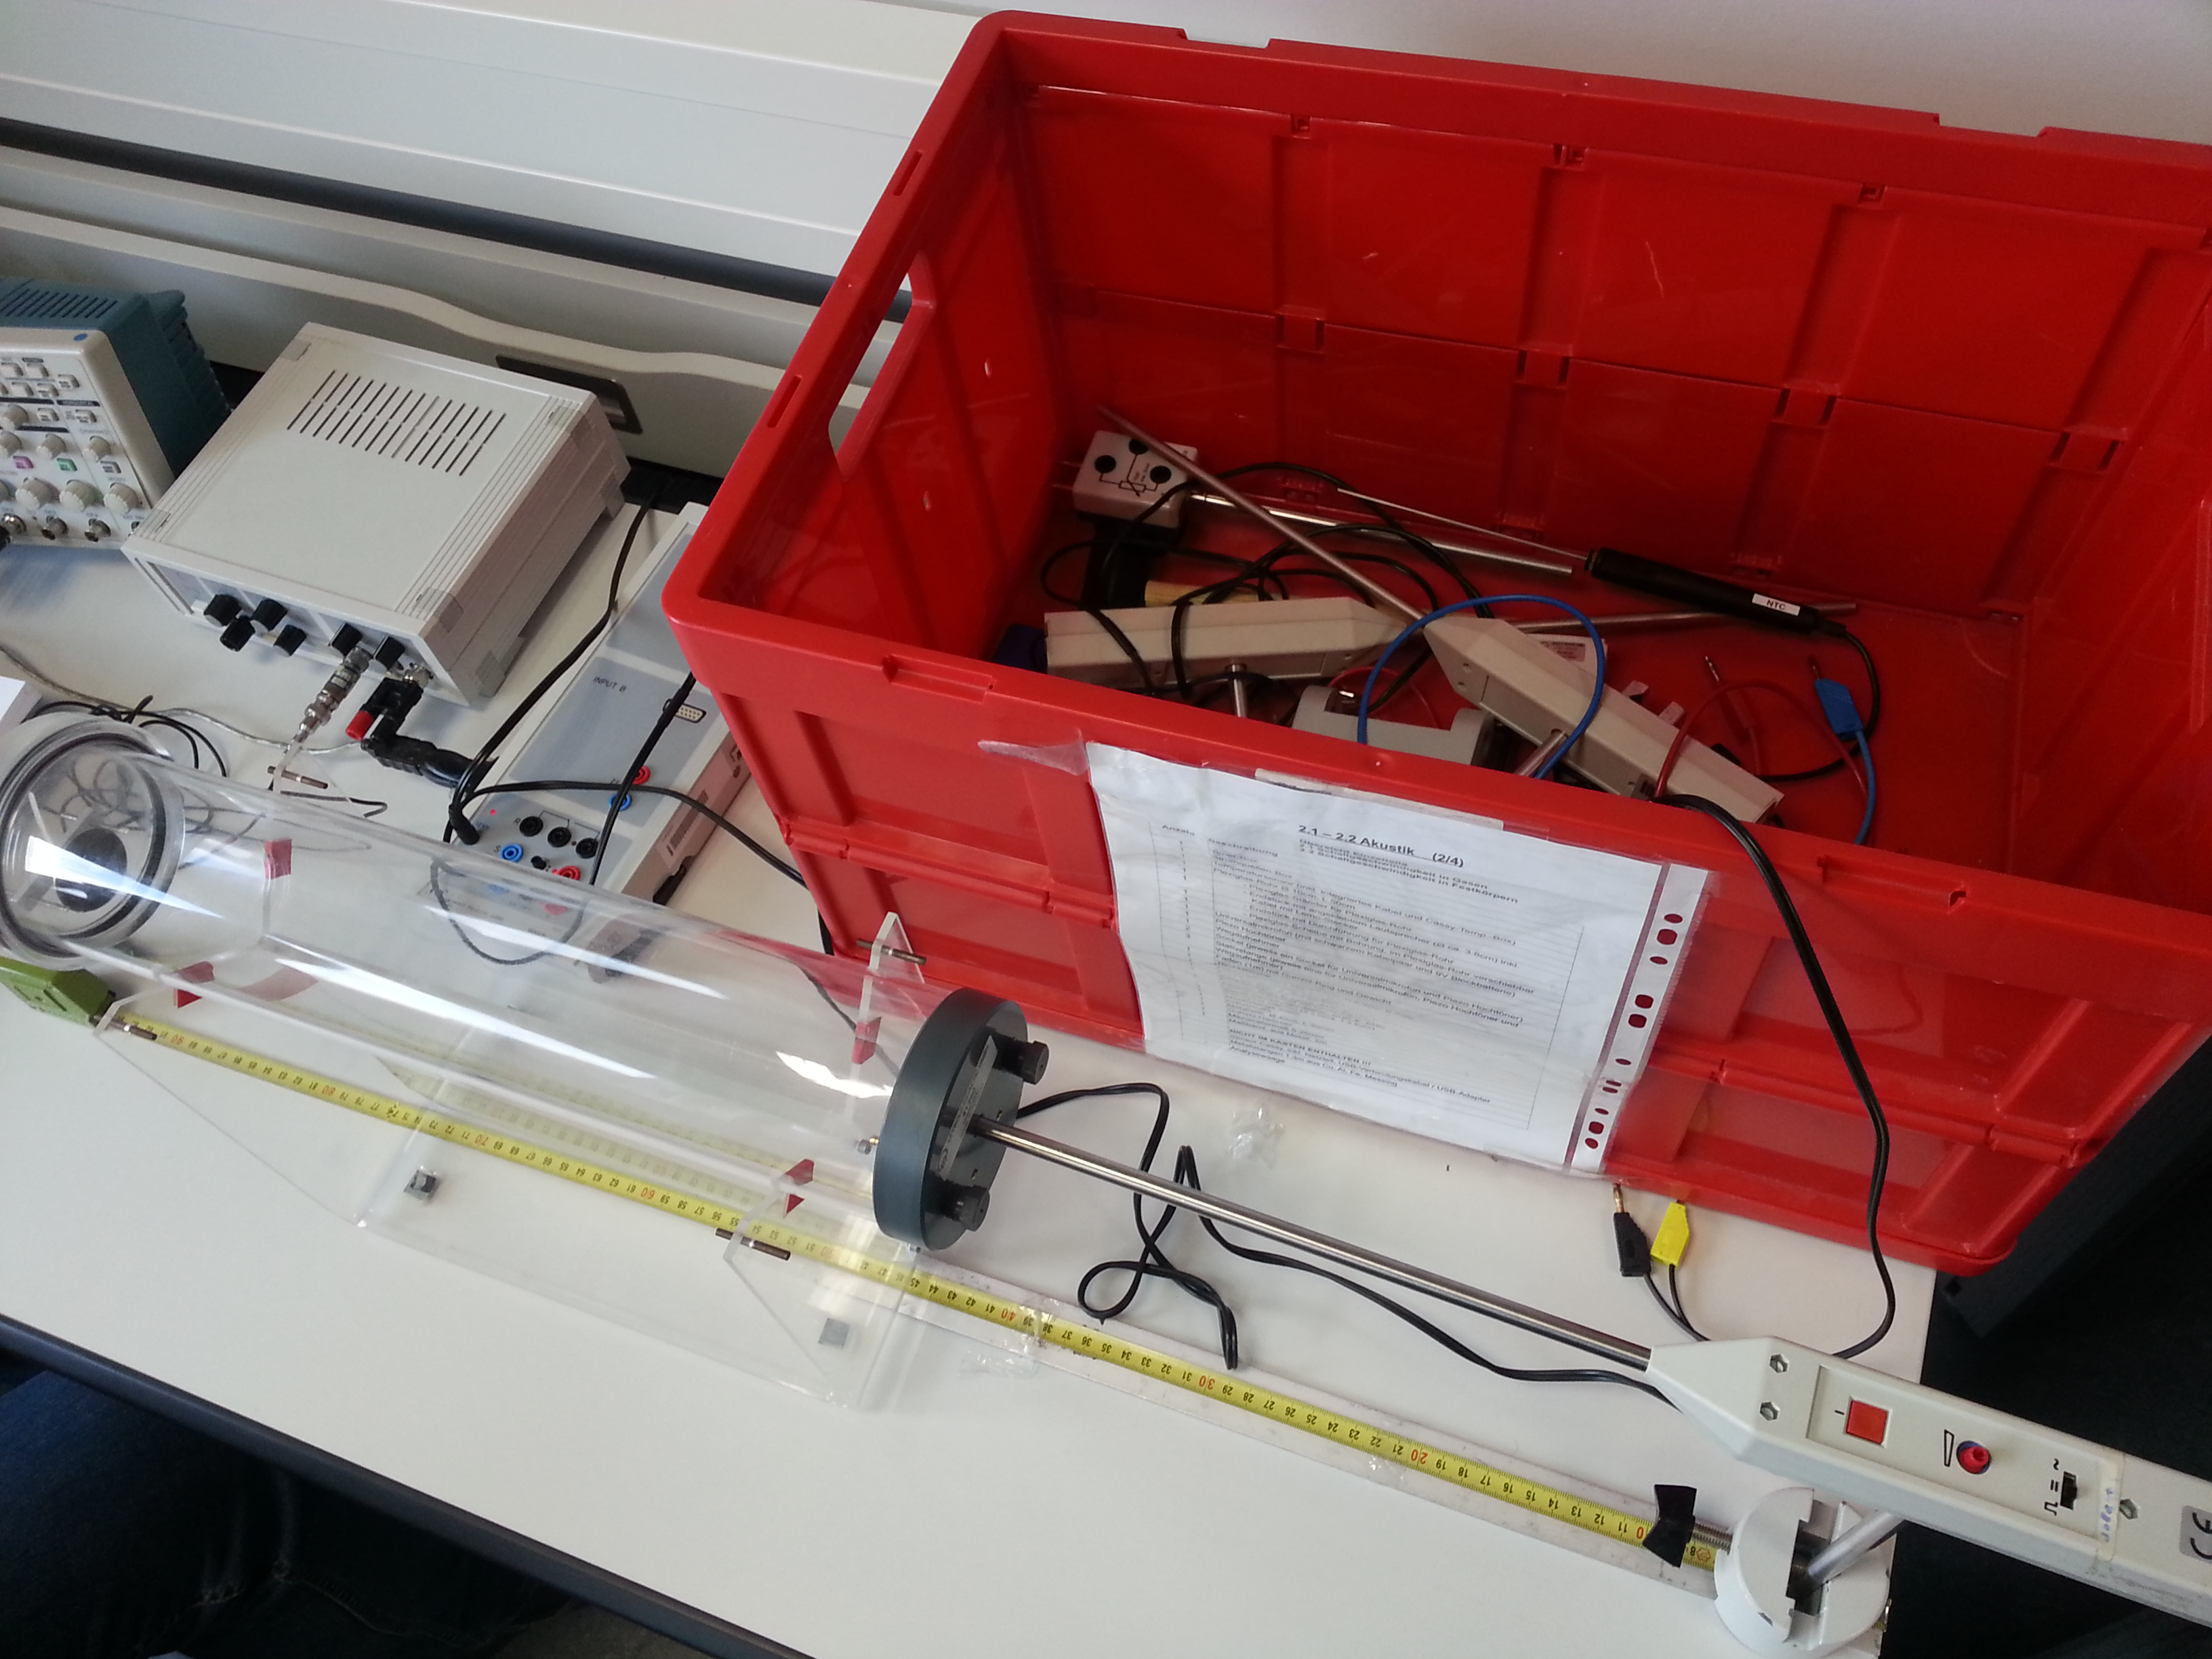
\includegraphics[scale=0.1]{Bilder/Druckknoten-Messung3.jpg}
\caption{Versuchsaufbau für die Bestimmung der Schallgeschwindigkeit über die Vermessung einer stehenden Welle}
\end{figure}
Durchführung:\newline
Wir messen alle 0.5$\,$cm angefangen bei 2.5$\,$cm (gemessen vom Anfang der Schiene). Die Umrechnung von n in m lautet also wie folgt:
\begin{equation}
l = (0.025 + n\cdot 0.005) - 0.425
\end{equation}
wobei die 42.5$\,$cm die Länge des Rohres beschreibt, wie unter Geräte angegeben.
Die sich so ergebenen Daten sehen wie folgt aus:
\begin{figure}[H]
\centering
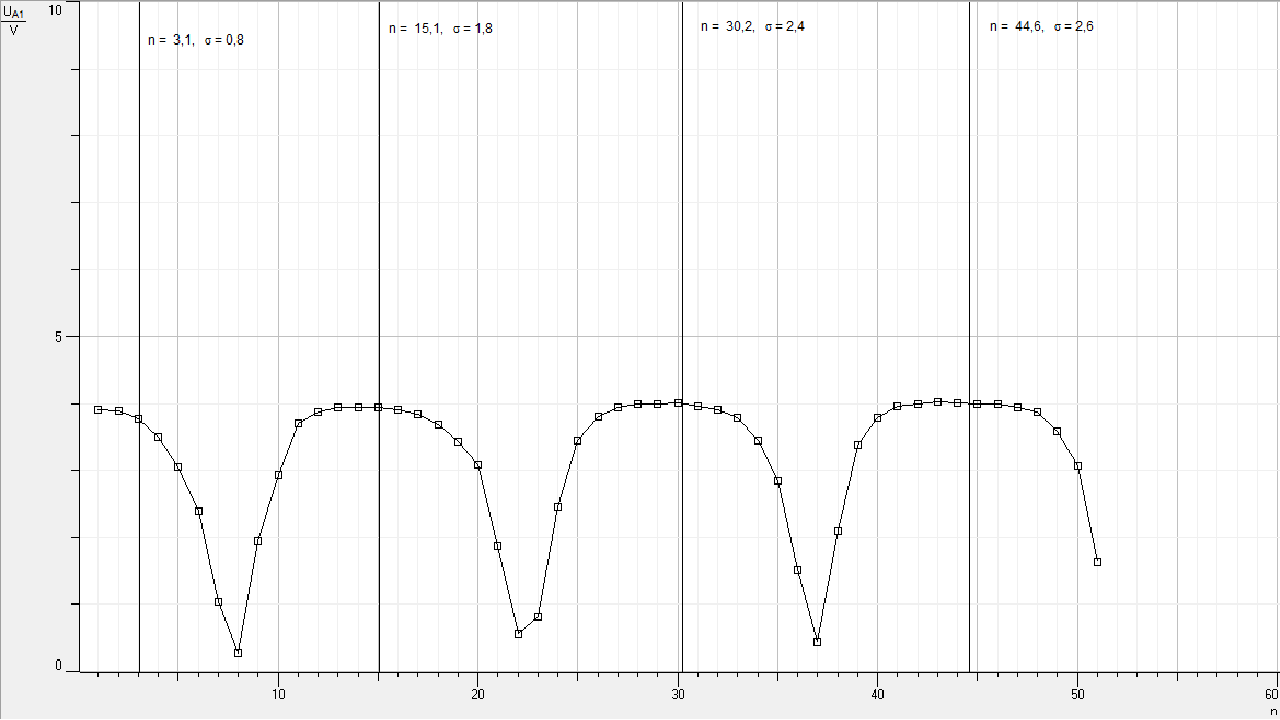
\includegraphics[scale=0.3]{Bilder/baeuche.png}
\caption{Amplitude des Schalldrucks aufgetragen gegen eingeführte Länge des Richtmikrofons (in n - Umrechnung siehe oben)}
\end{figure}
Wir haben leider wenig Punkte bei den Knoten, daher werden wir für unsere Lineare Regression nur unsere Peaks betrachten. Diese bestimmen wir mit der Peaksschwerpunktfunktion von Cassy.
Die sich daraus ergebenen Daten sind unter Rohdaten aufgeführt.

\subsection{Versuchsauswertung}

\subsubsection{Rohdaten}
\begin{table}[H]
\begin{tabular}{c|c|c}
Position Bauch N & Messpunkt n & Länge [m] \\ 
\hline 
1.5 & 1 & 0.395 \\ 
2.5 & 15 & 0.325 \\ 
3.5 & 30 & 0.25 \\ 
4.5 & 45 & 0.175 \\ 
\end{tabular}
\caption{Druckbäuche für $f = 2400\,$Hz, mit $\sigma_l = 0.0028\,$m}
\end{table}
\subsubsection{Transformation der Rohdaten}
Mit den oben genannten Rohdaten führen wir jetzt eine Lineare Regression durch. Die Steigung der Linearen Regression gibt uns $\frac{\lambda}{2}$ zurück und beträgt $0.0735\,$m. Unsere Lineare Regression sieht wie folgt aus:
\begin{figure}[H]
\centering
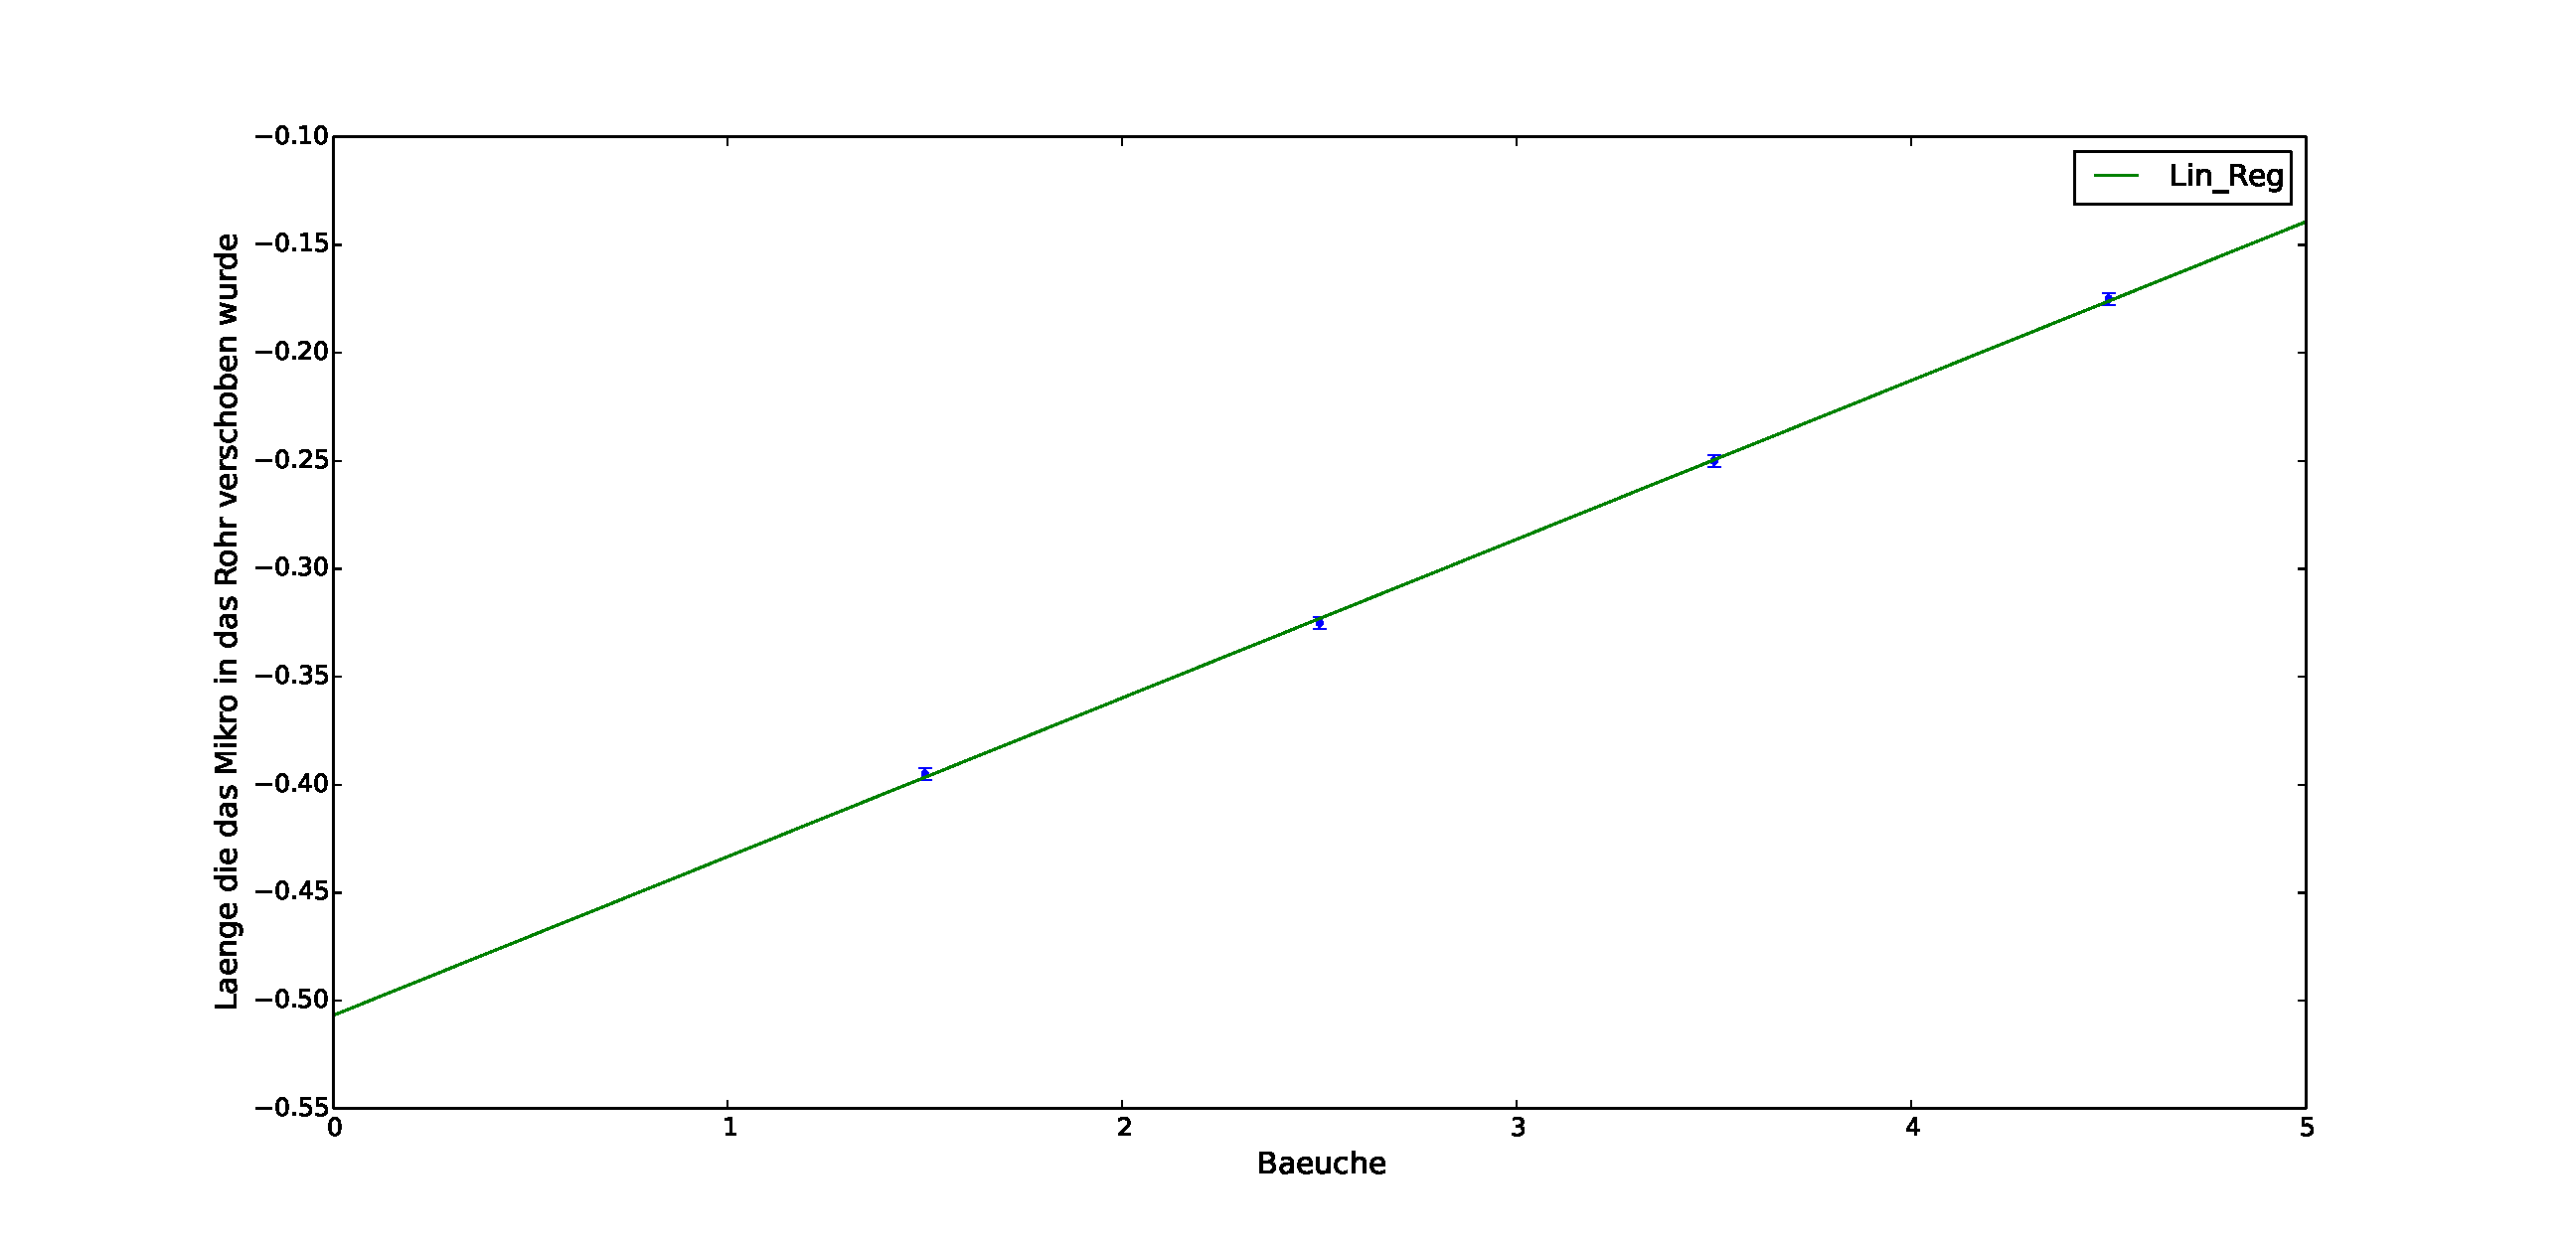
\includegraphics[scale=0.3]{Bilder/linreg_stehende_welle.eps}
\caption{Lineare Regression der 4 oben genannten Peaks, die Steigung beträgt $\frac{\lambda}{2}$}
\end{figure}
Wir haben dabei ein $\chi^2 = 0.47$ erreicht.
Unser Residuenplot dazu sieht wie folgt aus:
\begin{figure}[H]
\centering
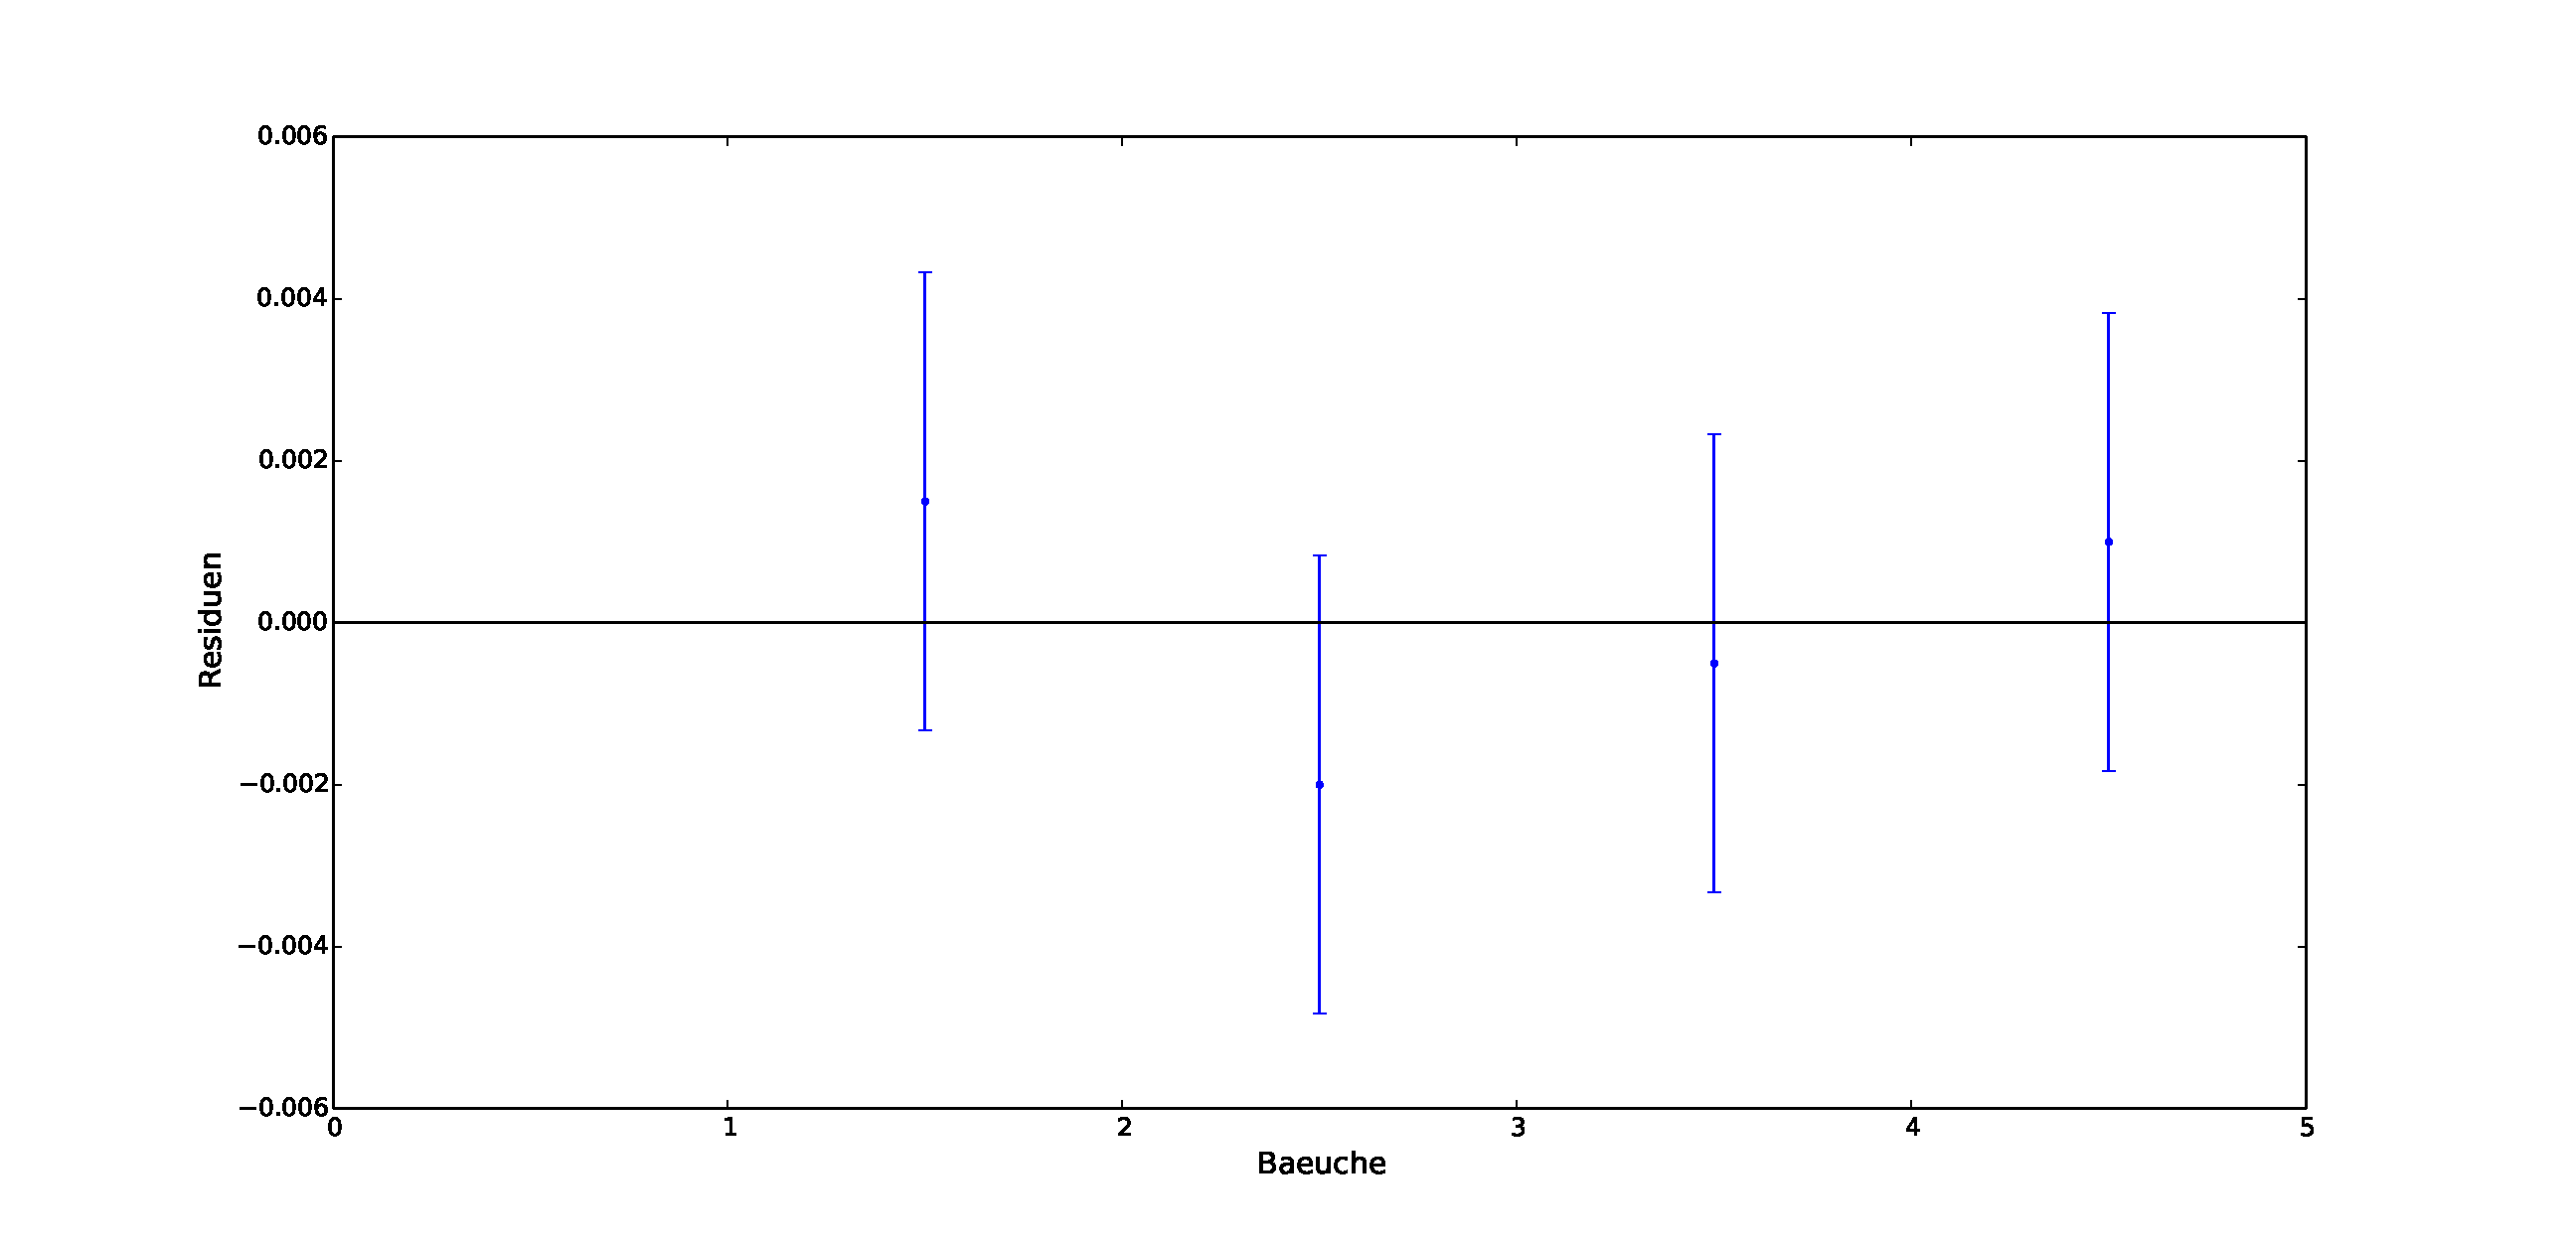
\includegraphics[scale=0.3]{Bilder/residuen_stehende_welle.eps}
\caption{Residuenplot (Daten - Fit) mit den jeweiligen Fehlern}
\end{figure}
Alle Werte liegen mit ihren Fehlern in einem Abstand kleiner als $\sigma$ von 0 entfernt. Die Werte sind gleichverteilt um 0 gestreut und es lässt sich keine Systematik erkennen.\newline
Um auf unseren Wert für $v$ zu kommen müssen wir die eingestellte Frequenz $f = 2400\,$Hz und die mit dem Faktor 2 multiplizierte Steigung (wir erinnern uns, dass die Steigung der Linearen Regression nur $\frac{\lambda}{2}$ zurückgab) der Linearen Regression in die am Anfang dieses Kapitels eingeführte Gleichung
\begin{equation*}
v = \lambda\cdot f
\end{equation*}
einsetzen. So erhalten wir einen Wert für $v = 352.8\,\frac{m}{s}$.
Um den Fehler auf $v$ zu erhalten, müssen wir $\sigma_{\lambda}$ und $\sigma_f$ fortpflanzen.
\begin{equation}
\sigma_{v} = \sqrt{f^2\cdot\sigma_{\lambda}^2 + \lambda^2\cdot\sigma_{f}^2}
\end{equation}
mit $\sigma_{\lambda} = 0.0025\,$m (aus Ausgabe der Linearen Regression.)
Daraus ergibt sich für unser Ergebnis, dass die Schallgeschwindigkeit $v_{Schall} = 352.8 \pm 4.5\,\frac{m}{s}$ beträgt.

\subsection{Fazit}
Unser Ergebnis für die Schallgeschwindigkeit liegt innerhalb von 2$\sigma_{v}$ über dem Literaturwert (bei T$ = 20^{\circ}\,$C beträgt die Schallgeschwindigkeit $v = 343.\,\frac{m}{s}$, umgerechnet für T$ = 22.6^{\circ}\,$C mit $v = v_0\cdot\sqrt{\frac{T}{T_0}}$, $v = 344.98\,\frac{m}{s}$). Wir erklären uns diese Abweichung durch die fehlenden Werte für die Druckknoten der stehenden Welle in der Linearen Regression. Ansonsten sind wir sowohl mit unserer Anpassung ($\chi^2 = 0.47$) als auch mit der um 0 gleichverteilt gestreuten Residuen zufrieden.
\end{document}